\section{Ejercicio 3}

Peso asignado: 8.

\subsection{Problema}

Se presenta una situación en la cual se tiene una cantidad \textbf{H} de puntos en un espacio bidimencional
$<xh_1,yh_1>,...,<xh_H,yh_H>$ de edificios historicos de una ciudad y \textbf{E} puntos de edificios
enemigos $<xe_1,ye_1>,...,<xe_E,ye_E>$.

Dados esos parámetros de entrada se quiere calcular la máxima cantidad de puntos históricos que podría cubrir
una muralla que forme un polígono convexo de forma que no contenga ningún edificio enemigo.

\subsection{Solución}

\subsubsection{Explicación}

En primera instancia, se guardan los puntos de entrada en dos vectores distintos.

Se sabe que se quiere armar un polígono convexo como muralla alrededor de los puntos históricos y que los
edificios que están en los vértices de tal muralla, están también dentro de la muralla. Por lo tanto, lo
que se quiere es formar un \textit{Convex Hull} de subconjunto de puntos históricos de forma tal que no
contenga edificios enemigos y se maximice la cantidad de puntos históricos.

Como el \textit{Convex Hull} que se quiere armar puede ser triangulado, es decir, descompuesto en triángulos
según un nodo origen con el cual se traza un segmento hacia todos los otros nodos, vamos a ir armando el
\textit{Convex Hull} uniendo triángulos, que no es más que agregar un vértice al polígono de la siguiente forma:

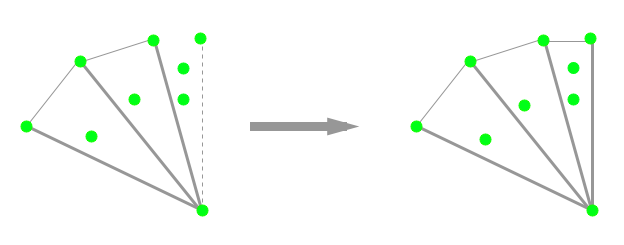
\includegraphics[scale=0.5]{img/ej31.png}

Como no hay nunca tres vértices alineados, toda tripla de vértices generará un triángulo válido.

Ahora bien, mientras se van agregando vértices hay que chequear que no se haya agregado un
triángulo que contenga enemigos. Además habrá que ver que el nuevo polígono es convexo y cuántos lugares
históricos fueron agregados de forma de mantener la información que se necesita para llegar a la solución final:

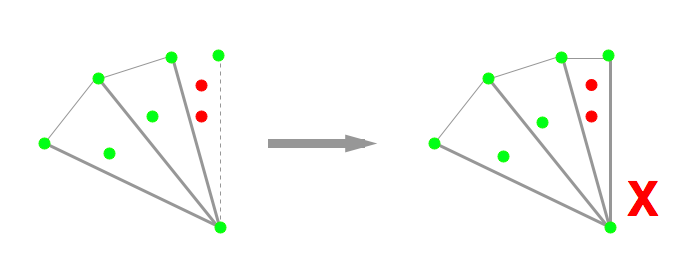
\includegraphics[scale=0.5]{img/ej32.png}

Como consecuencia de todo lo anterior, nuestro algoritmo precomputa desde el inicio para cada tripla de
vértices de puntos históricos distintos, la cantidad de puntos históricos y la cantidad de edificios enemigos dentro del
triángulo que generan (sin contarse a ellos mismos):

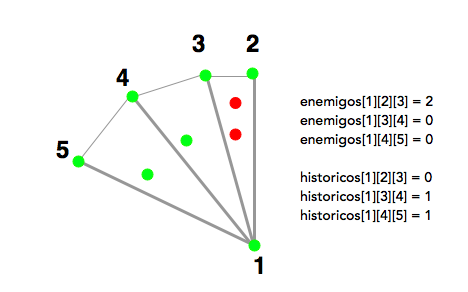
\includegraphics[scale=0.5]{img/ej33.png}

Teniendo toda esa información, vamos a querer armar para cada vértice $P$, un \textit{Convex Hull} a partir de $P$
si solo se consideran los vértices $V$ de puntos históricos que cumplan: $V.y > P.y \cup (V.y = P.y \cap V.x > P.x)$ con 
la cantidad máxima posible de lugares históricos y sin edificios enemigos. 
Es decir, solo contando los vértices que estén más arriba que $P$ o que tengan la misma coordenada $y$ pero estén más a
la derecha.

Esta restricción nos permite hacer un Graham Scan, ya que el algoritmo comienza tomando el punto más abajo y de
entre ellos el de más a la izquierda. Entonces si solo se consideran los puntos que cumplen la condición anterior,
se producirá un \textit{Convex Hull}. 

Notar que si probamos a todos los vértices posibles como el vértice de más abajo y más a la izquierda de entre ellos,
en algún momento el algoritmo va a considerar el vértice a partir del cual se forma el \textit{Convex Hull} buscado.

Sin embargo no es exactamente un Graham Scan lo que se va a hacer.

En primera instancia, ordenamos los vértices según el ángulo que forman con $P$ en sentido antihorario:

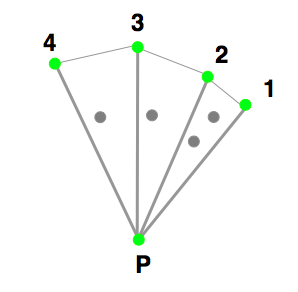
\includegraphics[scale=0.5]{img/ej34.png}

A medida que vamos armando el polígono convexo, hay que fijarse si se introducen edificios enemigos y cuántos
puntos históricos se van agregando. A su vez, como cualquier triángulo puede contener enemigos, no alcanza
con obtener un \textit{Convex Hull} para todos los puntos, sino que vamos a ir agregando triángulos gradualmente.

Como cada triángulo se determina mediante los dos puntos históricos diferentes a $P$, guardamos en un arreglo 
bidimensional $dp$ la máxima cantidad de puntos históricos que podemos tener sin contener enemigos en el polígono, si 
ese triángulo es el primero que agregamos (y solo agregamos triángulos en sentido horario). De esa manera, vamos 
chequeando si se pueden agregar vértices con un índice menor:

\centerline{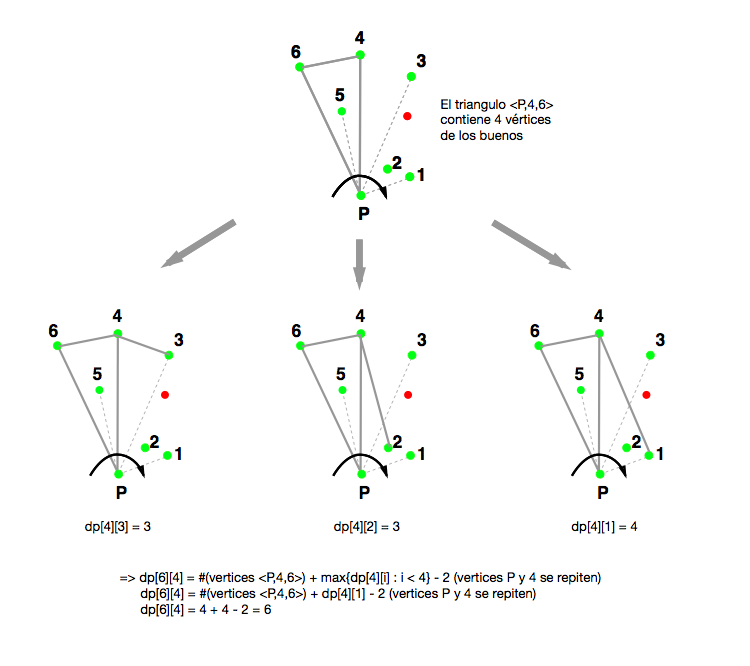
\includegraphics[scale=0.7]{img/ej35.png}}

Como vemos en la figura anterior, a partir de $i_1,...,i_n$ los puntos históricos que cumplen
$i_k.y > P.y \cup (i_k.y = P.y \cap i_k.x > P.x)$ ordenados en sentido antihorario según $P$, se definirán los
valores de $dp$. 

Sean $i_t, i_j \cap t > j$, si el primer triángulo que agrego es $<P,i_t,i_j>$ y los vértices que puedo agregar
para formar nuevos triángulos los agrego en sentido horario, tengo que buscar para cada $i_k \cap j > k$, cuántos
vértices podría agregarle al polígono si el primer triángulo que agrego es $<P,i_j,i_k>$, es decir $dp[j][k]$.
Si el triángulo $<P,i_t,i_j>$ contiene edificios enemigos, $dp[t][j] = 0$, en caso contrario:

\begin{equation*}
\begin{split}
    dp[t][j] & = \#\{ puntos\_historicos \in Triangulo(<P,i_t,i_j>)\} + 3 + \\
    & \max_{ i_k : j > k \cap valido(t,j,k) } \{dp[j][k]-2\} \\
    & = \#\{ k : k \in \{i_1,...,i_n\} \cap k \neq i \cap k \neq j \cap k \in Triangulo(<P,i_t,i_j>)\} + 3 + \\
    & \max_{ i_k : j > k \cap valido(t,j,k) } \{dp[j][k]-2\}
\end{split}
\end{equation*}

Donde $valido(t,j,k)$ es verdadero si y solo si el triángulo generado por $P, i_j, i_k$ no contiene edificios enemigos
y al unir el triángulo $P, i_t, i_j$ al $P, i_j, i_k$, el polígono sigue siendo convexo.

Notar que a $dp[j][k]$ se le resta 2 en la ecuación debido a que al unir el triángulo $P, i_t, i_j$ al $P, i_j, i_k$,
se están contando los puntos históricos $P, i_j$ dos veces.

\subsubsection{Pseudocódigo y correctitud}

En esta sección se detallarán las clases y los métodos importantes de la solución.

\subsubsection*{Clase punto}

Un Punto contendrá sus coordenadas $x,y$ ya que trabajamos sobre un espacio bidimencional. Asi mismo definimos
la igualdad de puntos por la igualdad de sus coordenadas. La suma y resta de puntos se define como la suma y resta
de sus coordenadas respectivamente. El producto crus $P \times Q = P_x * Q_y - Q_x * P_y$.

\subsubsection*{Clase segmento}

Un segmento contendrá simplemente un Punto origen $a$ y un Punto destino $b$. Asi se definen las funciones:

\begin{algorithm}[H]
	\caption{\textit{ContieneSegmentoPunto}}
	\Input{ Segmento $S$, Punto $P$ }
	\Output{ Bool }
	\Return{ValorAbsoluto((S.b-P) $\times$ (P-a)) $<$ epsilon \&\& \\
	min(S.a.x,S.b.x) - epsilon $\leq$ P.x \&\& P.x $\leq$ max(S.a.x, S.b.x) + epsilon \&\& \\
	min(S.a.y,S.b.y) - epsilon $\leq$ P.y \&\& P.y $\leq$ max(S.a.y, S.b.y) + epsilon}
\end{algorithm}

Es decir devuelve true si y solo si S.b-a y P-a son paralelos (y por lo tanto están en la misma recta infinita)
y además está dentro de los límites del segmento y no solo en la misma recta infinita.
Donde epsilon es una constante de valor positivo muy chico para prevenir errores de estabilidad numérica.

\begin{algorithm}[H]
	\caption{\textit{IntersecciónSegmentos}}
	\Input{ Segmento $S$, Segmento $Q$ }
	\Output{ Punto }
	Punto v1 = P.b - P.a \\
	Punto v2 = Q.b - Q.a \\
	bool paralelos = v1 $\times$ v2 == 0 \\
	\eIf{paralelos == false} {
		double alpha = (Q.a-a) $\times$ v2 / v1 $\times$ v2 \\
		Punto intersection = a + Punto(alpha * v1.x, alpha * v1.y)
		\If {S.ContieneSegmentoPunto(intersection) \&\& Q.ContieneSegmentoPunto(intersection))}{
			\Return{intersection}
		}
	}{
		\If {S.ContieneSegmentoPunto(Q.a))} {\Return{Q.a}}
		\If {S.ContieneSegmentoPunto(Q.b))} {\Return{Q.b}}
		\If {s.ContieneSegmentoPunto(a))} {\Return{a}}
		\If {s.ContieneSegmentoPunto(b))} {\Return{b}}
	}
	\Return{Null}
\end{algorithm}

Sabiendo que es más fácil hacer cuentas sobre rectas si tenemos la representación en formato $L(t)=a+t*(b-a)$ para
cada recta $L$ con puntos $a$ y $b$, obtenemos para ambos segmentos la resta $b-a$ y los guardamos en $v1$ y $v2$.
Lo que hace esta rutina es primero fijarse si las rectas son paralelas y como vimos en clase esto es verdadero
cuando $v1 \times v2$ es igual a 0. Si las rectas son paralelas, tienen intersección simplemente si alguna 
contiene un extremo de la otra. Si no son paralelas, también como vimos en clase, hay que buscar un alpha que
cumpla $alpha = (Q.a-a) \times v2 / v1 \times v2$ para encontrar la intersección entre las rectas si es que
fueran infinitas. Luego hay que fijarse si ambos segmentos contienen la intersección de las rectas infinitas
y si lo hacen, devolver la intersección.

\subsubsection*{Clase Triángulo}

Un triángulo se define mediante sus tres vértices extremos $a$, $b$ y $c$.
La operación importante para esta clase será:

\begin{algorithm}[H]
	\caption{\textit{ContieneTrianguloPunto}}
	\Input{ Triangulo $<a,b,c>>$, Punto $P$ }
	\Output{ Bool }
	double $leftmost\_x$ = min(a.x, min(b.x, c.x)) \\
	Segment $ray$ = Segment(Point($leftmost\_x$-1,p.y),p) \\
	int $intersections$ = 0 \\
	Segment $ab$ = Segment(a, b) \\
	Segment $bc$ = Segment(b, c) \\
	Segment $ca$ = Segment(c, a) \\
	\If {$ray$.InterseccionSegmentos($ab$) $\neq$ Null}{ $intersections$++ }
	\If {$ray$.InterseccionSegmentos($bc$) $\neq$ Null}{ $intersections$++ }
	\If {$ray$.InterseccionSegmentos($ca$) $\neq$ Null}{ $intersections$++ }
	\If {$ray$.ContieneSegmentoPunto(a))}{
		\If {b.y $<$ p.y}{ $intersections$ -= 1 }
		\If {c.y $<$ p.y}{ $intersections$ -= 1 }
	}
	\If {$ray$.ContieneSegmentoPunto(b))}{
		\If {a.y $<$ p.y}{ $intersections$ -= 1 }
		\If {c.y $<$ p.y}{ $intersections$ -= 1 }
	}
	\If {$ray$.ContieneSegmentoPunto(c))}{
		\If {a.y $<$ p.y}{ $intersections$ -= 1 }
		\If {b.y $<$ p.y}{ $intersections$ -= 1 }
	}
	\If {($ray$.ContieneSegmentoPunto(a) \&\& $ray$.ContieneSegmentoPunto(b)) $\|$ ($ray$.ContieneSegmentoPunto(a) \&\& $ray$.ContieneSegmentoPunto(c)) $\|$ ($ray$.ContieneSegmentoPunto(c) \&\& $ray$.ContieneSegmentoPunto(b))}{
		$intersections$ = 0
	}
	\Return{$intersections$ == 1 $\|$ $ab$.ContieneSegmentoPunto(p) $\|$ $bc$.ContieneSegmentoPunto(p) $\|$ $ca$.ContieneSegmentoPunto(p)}
\end{algorithm}

Lo primero que hacemos es calcular de los tres puntos del triángulo la menor coordenada $x$. A ese valor se
le resta 1 para asegurarse que se empieza desde un punto fuera del triángulo. Luego se crea un Segmento $ray$
horizontal desde $<leftmost\_x-1, p.y>$ hasta $P$. Como vimos en clase, el punto $P$ estará contenido en el 
triángulo si interseca con el mismo una cantidad impar de veces. Como no puede intersecarlo 3 veces, el punto
está adentro si hay exactamente una intersección con alguno de los segmentos $ab$, $bc$ o $ca$.
Luego hacemos un chequeo de casos borde. Puede pasar que $ray$ tenga una intersección con uno o dos vértices
del triángulo (tres no porque los tres vértices de un triángulo no pueden estar alineados). Como $ray$ es un
segmento horizontal, los casos posibles (según la coordenada $y$ de los tres puntos) son: 

\centerline{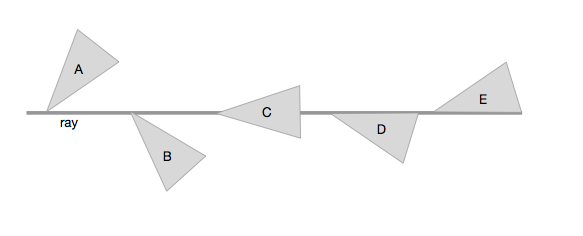
\includegraphics[scale=0.7]{img/ej36.png}}

Entonces lo que el algoritmo hace según los casos anteriores (entre los \textit{if} de las líneas 16-39) es:
\begin{itemize}
\item[A:] $intersections$ termina siendo 2 ya que se cuenta la misma dos veces, lo cual esta bien porque
no se quiere considerar que $ray$ entró en el triángulo.
\item[B:] $intersections$ termina siendo 0, lo cual esta bien porque
no se quiere considerar que $ray$ entró en el triángulo.
\item[C:] se cuenta el vértice como 1 intersección ya que se quiere considerar que $ray$ entró en el triángulo.
\item[D:] $intersections$ termina siendo 0 porque $ray$ interseca con dos vértices del triángulo, por lo
tanto la salida será true si y solo si el punto $P$ está adentro de uno de los bordes.
\item[E:] idem caso D.
\end{itemize}

Notar que todo lo anterior sirve si el punto no está incluido en alguno de los lados del triángulo, por este
motivo, si el punto esta contenido en los segmentos $ab, bc$ ó $ca$, devolvemos true (incluyendo el caso
en el que el punto sea uno de los vértices del triángulo).

\subsubsection*{Resolución del problema}

\begin{algorithm}[H]
	\caption{\textit{MaximosPuntosHistoricosEnMurallaConvexa}}
	\Input{ int $H$, int $E$, $vector<int>$ $historical\_places$, $vector<int>$ $enemy\_places$ }
	\Output{ int }

	$vector<vector<vector<int>>>$ $historical\_places\_in\_triangle$ = vector tridimencional de $H \times H \times H$ \\
	$vector<vector<vector<int>>>$ $enemy\_places\_in\_triangle$ = vector tridimencional de $H \times H \times H$

	\For {cada tripla de int $i,j,k$ diferentes entre 0 y $H-1$} {
        Punto $pi$ = $historical\_places$[i] \\
        Punto $pj$ = $historical\_places$[j] \\
        Punto $pk$ = $historical\_places$[k] \\
        \For {cada $l$ diferente a $i,j,k$ entre 0 y $H-1$} {
            Punto $pl$ = $historical\_places$[$l$] \\
            \If{Triangulo($pi,pj,pk$).ContienePuntoTriangulo(pl)}{
                $historical\_places\_in\_triangle$[i][j][k]++
            }
        }
        \For {int $l$ = 0 hasta $E-1$} {
            Punto $pl$ = $enemy\_places$[$l$] \\
            \If{Triangulo($pi,pj,pk$).ContienePuntoTriangulo(pl)}{
                $enemy\_places\_in\_triangle$[i][j][k]++
            }
        }
    }

	int $ans$ = min(2, $H$) \\
	\For{cada $i$ entre 0 y $H-1$}{
	    $ans$ = max($ans$, MaximosPuntosHistoricosDesde($i$, $H$, $E$, $historical\_places$, $enemy\_places$))
	}

	\Return{$ans$}
\end{algorithm}

Esta es la función principal del problema, tal como pide el enunciado recibe dos enteros $H,E$ con la cantidad
de puntos históricos y edificios enemigos y dos vectores $historical\_places$ y $enemy\_places$ con las coordenadas
de los mismos.
Con ellos, calcula y devuelve la máxima cantidad de puntos históricos que puede contener una
muralla convexa sin edificios enemigos dentro.

El algoritmo comienza declarando dos vectores tridimencionales $historical\_places\_in\_triangle$ y \\
$enemy\_places\_in\_triangle$ que contendrán para cada tripla de puntos diferentes, la cantidad de puntos históricos
y la cantidad de puntos enemigos dentro del triángulo que determina la tripla.
Luego el \textit{For} de las líneas 3-19 se encarga justamente de tomar triplas de tres puntos diferentes,
crear un triángulo y fijarse para cada punto histórico y edificio enemigo si está contenido en el triángulo, asi
calculando los valores de los dos vectores.

La línea 20 inicializa $ans$ como min(2, $H$) por el caso de que hayan menos de tres puntos hitóricos en la ciudad
y entonces se tenga que contruir una muralla para 0, 1 ó 2 puntos históricos (cosa que siempre es posible).

Finalmente el \textit{For} de las líneas 21-23 calcula para cada punto histórico, la respuesta al problema
si es que la muralla fuera armada a partir de ese punto uniéndolo mediante triángulos a otros puntos históricos
con coordenada $y$ mayor o coordenada $y$ equivalente y mayor coordenada $x$, todo esto tal como fue explicado
en la sección de \textbf{Explicación}. La respuesta es el máximo de estos valores, porque en algún momento el ciclo
toma el punto para el que se formará el \textit{Convex Hull} buscado (porque se prueba a partir de todos los puntos).

\bigskip

\begin{algorithm}[H]
	\caption{\textit{MaximosPuntosHistoricosDesde}}
	\Input{ int $ref\_point, $int $H$, int $E$, $vector<int>$ $historical\_places$, $vector<int>$ $enemy\_places$ }
	\Output{ int }
	Punto p = $historical\_places$[$ref\_point$] \\

    $vector<int>$ $valid\_historical\_places$ = \{ $i$ : $i$ entre 0 y $H-1$ y cumple que $historical\_places$[i] está más arriba que $p$ o tiene la misma coordenada $y$ pero mayor coordenada $x$ \} \\
    
    Ordenar $valid\_historical\_places$ según el ángulo de los puntos capturados con $P$ en sentido antihorario \\
    
    int V = $valid\_historical\_places$.size() \\
    $vector< vector<int> > dp$ = vector bidimencional relleno de 0 de tamaño $V \times V$ \\

    \For {cada $i$ de 0 a $V-1$} {
        int hi = $valid\_historical\_places$[i] \\
        \For {cada $j$ de 0 a $i-1$} {
            int hj = $valid\_historical\_places$[j] \\
            \If {$enemy\_places\_in\_triangle$[$ref\_point$][hi][hj] $\leq$ 0}{
	            int $h\_places$ = 3 + $historical\_places\_in\_triangle$[$ref\_point$][hi][hj] \\
	            $dp$[i][j] = $h\_places$ \\
	            \For {cada $k$ de 0 a $j-1$} {
	                int hk = $valid\_historical\_places$[k] \\
	                Punto r = $historical\_places$[hj] \\
	                Punto p = $historical\_places$[hi] \\
	                Punto q = $historical\_places$[hk] \\
	                bool $sigue\_convexo$ = (p-r) $\times$ (q-r) $>$ 0 \\
	                bool $sin\_enemigos$ = $enemy\_places\_in\_triangle$[$ref\_point$][hj][hk] == 0 \\
	                \If {$sigue\_convexo$ \&\& $sin\_enemigos$}{
						$dp$[i][j] = max($dp$[i][j], $h\_places$ + $dp$[j][k] - 2)
					}
	            }
            }
        }
    }

    \Return{$\max_{i,j}\{$dp$[i][j]\}$}
\end{algorithm}

Como fue explicado anteriormente, se quiere armar un \textit{Convex Hull} como si el punto con índice $ref\_point$
(que llamamos $P$) fuera el de más abajo y de entre ellos el de más a la izquierda.

Primero se filtran los puntos históricos que están arriba o tiene igual coordenada $y$ y mayor $x$ y se los guarda en 
el vector $valid\_historical\_places$.

Luego, de la misma manera que el Graham Scan se ordenan esos puntos según el ángulo que forman con $P$ (notar que no
hay dos con el mismo ángulo porque se garantiza que no hay tres vértices alineados). Esto se hace como en cualquier
algoritmo de ordenamiento pero definiendo el orden de manera que dos puntos $Q, R$ cumplen $Q < R$ si y solo si
$(Q-P) \times (R-P) > 0$. De esa manera ordenamos de menor a mayor para obtener los puntos en sentido antihorario.

Como paso siguiente, se crea el vector bidimencional $dp$ que para $i > j$, $dp[i][j]$ contiene la máxima cantidad de 
puntos históricos que podemos tener en el polígono convexo triangulado sin contener enemigos, si
ese triángulo es el primero que agregamos (y solo agregamos triángulos en sentido horario).

De esa manera, y como fue explicado antes, entre las líneas 6-26 rellenamos $dp$ tal que:
\begin{equation*}
\begin{split}
    dp[i][j] & = \#\{ puntos\;historicos \in Triangulo(<P,valid\_historical\_places[i],valid\_historical\_places[j]>)\} + 3 + \\
    & \max_{ k : j > k \cap valido(i,j,k) } \{dp[j][k]-2\}
\end{split}
\end{equation*}

Donde $valido(t,j,k)$ es verdadero si y solo si:
\begin{itemize}
\item El triángulo generado por $<P, valid\_historical\_places[j], valid\_historical\_places[k]>$ no contiene edificios enemigos
cosa que se chequea en la línea 19.
\item Al unir el triángulo $<P, valid\_historical\_places[i], valid\_historical\_places[j]>$ al \\
$<P, valid\_historical\_places[j], valid\_historical\_places[k]>$, el polígono sigue siendo convexo
(lo cual comprobamos en la línea 18).
\end{itemize}

Finalmente devolvemos $\max_{i,j}\{dp[i][j]\}$, es decir, la cantidad de puntos históricos del \textit{Convex Hull} a partir de $P$
sin enemigos que contiene la máxima cantidad de puntos históricos.

\subsubsection{Complejidad}

\subsection{Casos de test}